\chapter{RISC-V} % Main chapter title
\label{RISC-V} % For referencing the chapter elsewhere, use \ref{Chapter1} 

\section{Einleitung}
\emph{RISC-V} ist eine offene Befehlssatzarchitektur, die 2010 von Entwicklern an der University of California, Berkeley vorgestellt wurde. Sie basiert auf der RISC (reduced instruction set computing) Design\textit{philosophie}. 

\paragraph{RISC.} Die Grundgedanke der RISC-Architekturen ist, dass die Anzahl ein Maschinenbefehl möglichst wenige Taktzyklen in der Ausführung benötigt. Damit grenzt sich RISC zu CISC (complex instruction set computing)-Systemen ab, die komplexe Instruktionen beinhalten, die viele Taktzyklen zur Ausführung benötigen können. RISC-Programme bestehen daher üblicherweise aus mehr Maschinenbefehlen, die aber tendenziell geringere Ausführungszeit benötigen.

%\textit{Der \textit{reduced instruction} ist insofern irreführend, da die Menge der verfügbaren Maschinenoperationen nicht zwangsweise geringer als in vergleichbaren CISC-Architekturen ist.
%}

Auch wenn der Begriff \textit{reduced instruction} sich nicht zwangsweise auf die Menge der verfügbaren Maschinenoperationen bezieht, bestehen RISC-Designs in der Praxis dennoch meist aus weniger Befehlen. Ein Vorteil, insbesondere im Hinblick auf das vorliegende Projekt, liegt darin, dass RISC Architekturen in der Regel eine weniger komplizierte Verschaltung erfordern und sind daher einfacher zu implementieren sind. \footnote{\url{https://www.elektronik-kompendium.de/sites/com/0412281.htm}} 

%Eine Befehlssatzarchitektur definiert den Befehlssatz einer CPU. Sie spezifiziert u. a., welche Maschinenbefehle eine CPU verarbeiten können muss, was genau ihre Ausführung bewirkt wie sie mit dem Speicher interagiert und definiert und wie definiert CPU eigene Speicherbänke (Register). Sie stellt damit die Schnittstelle zwischen der Hardware und Software einer Maschine dar. Mithilfe einer solchen einheitlichen Schnittstelle kann Software ohne Kenntnis der zugrunde liegenden Hardware Software für eine Maschine programmieren.

%Von der Befehlssatzarchitektur abzugrenzen ist die Mikroarchitektur, die die Implementierung des Befehlssatzes auf einem Chip bestimmt.

%Für dieses Projekt wurde der RISC-V Befehlssatz übernommen, und eine eigene Hardware-Implementierung, die die Befehlssatzspezifikation von RISC-V erfüllt, entwickelt.

%----------------------------------------------------------------------------------------
\section{Architektur}

\subsection{Speicherarchitektur}
RISC-V ist als \textit{load-store}-Architektur entworfen. Arithmetische und logische Instruktionen greifen daher nicht auf den Speicher zu, stattdessen werden alle Operanden vorher in der Registerbank abgelegt. Operationsergebnisse werden ebenfalls in Registern abgelegt. Speicherzugriffe werden ausschließlich mit \textit{load} bzw. \textit{store}-Befehlen realisiert.

\subsection{Register}
Die RISC-V Spezifikation definiert $31$ Integer Register $x1 - x31$. Zusätzlich existiert das \textit{zero}-Register $x0$, das eine konstante $0$ beinhaltet. Andere Register (Floating Point) können an dieser Stelle vernachlässigt werden, da sich die umgesetzte CPU auf Integerverarbeitung beschränkt.

\subsection{Maschinenbefehle}
RISC-V Maschinenbefehle sind in einer fixen Länge kodiert, die der Wortbreite der Architektur entspricht. Für RISC-V Architekturen sind die Wortbreiten $32, 64$ oder $128$bit vorgesehen.
%----------------------------------------------------------------------------------------

%----------------------------------------------------------------------------------------
\section{Verwendetes Instruktionssubset}

\paragraph{Erweiterungen.} Die RISC-V Architektur ist darauf ausgelegt, flexibel erweiterbar zu sein. Die Spezifikation definiert daher mehrere Teilmengen des allgemeinen Befehlssatzes. \citep[p. 4]{RISC}

Um die RISC-V Anforderungen zu erfüllen, muss eine Implementierung zumindest die Basisinstruktionen zur Integerverarbeitung umsetzen (Bezeichnung nach \mbox{RISC-V} Konvention: \textit{I})

Die allgemeine als \textit{General Purpose} bezeichnete Architektur enthält neben diesem Mindeststandard auch Befehle für Gleitkommaarithmetik (F) mit Double(D) oder Quad-Präzision (Q), für die Handhabung verschiedener Privilegierungen (P), atomare Befehle für die Verwaltung von Nebenläufigkeit (A) und seit der neusten Version 2.1 auch für Bitmanipulation (B), Vectoroperationen (V) und einigen mehr.

\paragraph{Verwendetes Subset.} In diesem Projekt wurde sich allerdings darauf beschränkt, eine einfache integerverarbeitende Mikroarchitektur umzusetzen. Als Wortbreite wurden 32bit gewählt. Die Bezeichnung des verwendeten Subsets lautet daher nach RISC-V Konvention \textit{RV32I}.
%----------------------------------------------------------------------------------------

%----------------------------------------------------------------------------------------
\section{RV32I}
Das verwendete Subset besteht aus $47$ verschiedenen Maschineninstruktionen.

\subsection{Instruktionsformate}
RV32I kennt vier verschiedene Typen, in denen Maschineninstruktionen enkodiert sein können: \textit{R-type}, \textit{I-Type}, \textit{S-type} und \textit{U-type} - Befehle. Dabei sind Opcode, sowie Ausgangsregister ($rs1$, $rs2$) und Zielregister ($rd$) der Operationen immer an der gleichen Stelle des Maschinenbefehls kodiert. Diese Einteilung in Instruktionstypen erleichtert die Dekodierung der Instruktionen und führt zu einer überschaubareren Verschaltung.

\begin{figure} [ht]
  \centering
  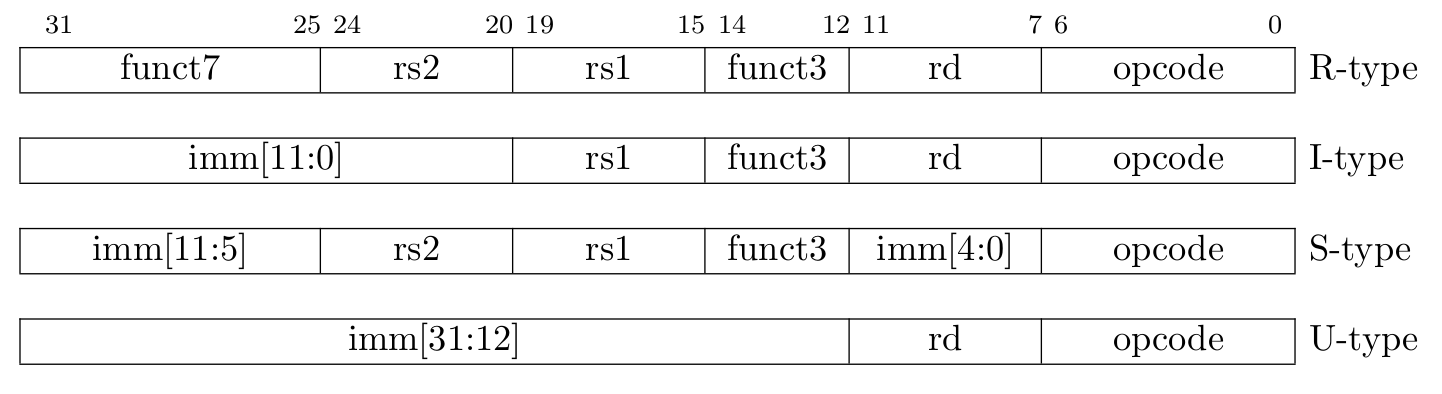
\includegraphics[width=0.95\textwidth]{Figures/instruction_formats}
  \caption{Instruktionsformate. Quelle: \citep[S. 11]{RISC}}
  \label{fig:instr_types}
\end{figure}

\paragraph{Immediate Varianten?}
...

\paragraph{R-Type.} Als R-Type sind Register-Instruktionen enkodiert, bei denen beide Operanden in Registern liegen.

\paragraph{I-Type.} Die I-Type-Kodierung ist für Instruktionen vorgesehen, bei denen ein konstanter Wert (\textit{Immediate}) mit einem Wert im Register verrechnet wird.

\paragraph{S-Type.}

\subsection{Maschineninstruktionen}
Die im R32I-Standard vorgesehenen Instruktionen können im einzelnen der Tabelle (im Anhang) zu entnommen werden.

Im folgenden sollen lediglich einige Instruktionen exemplarisch dargestellt werden.

\subsubsection{Integerverarbeitung}
Integer verarbeitende Instruktionen bestehen aus solchen, die eine Operation auf zwei Registerwerten ausführen (als R-Type kodiert) oder eine Operation auf einem Registerwert und einem Immediate (I-Type) ausführen. Das Operationsergebnis wird jeweils im Zielregister ($rd$) gespeichert.

In \ref{fig:addi} ist exemplarisch der \textit{ADDI}-Befehl zu sehen. Dieser soll einen im Maschinenbefehl kodierten Immediate-Wert mit einem einem Wert in einem bestimmten Register addieren und das Ergebnis anschließend in einem Zielregister speichern.
 
Dafür ist in der Maschineninstruktion der Opcode $0010011$ (bits $6 - 0$) kodiert, der die Information enthält, dass eine Immediateoperation durchgeführt werden soll. Die bits $14-12$ kodieren die \textit{funct3}, die die auszuführende Rechenoperation beschreibt (hier: $000$ für die Addition). Ferner ist das Zielregister $rd$, das Ausgangsregister $rs1$ und der Immediate-Wert (bit $31 - 20$) im Maschinenbefehl selbst kodiert.

\begin{figure} [ht]
  \centering
  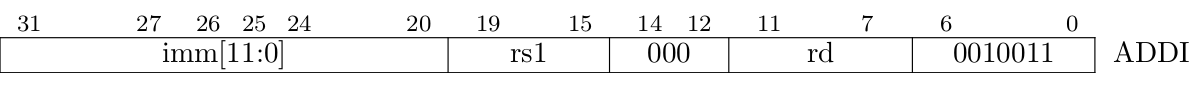
\includegraphics[width=0.95\textwidth]{Figures/ADDI}
  \caption{ADDI-Instruktion.}
  \label{fig:addi}
\end{figure}

In vergleichbarer Weise definiert RISC-V ferner Vergleichsinstruktionen (\textit{SLTI}), logische Operationen (\textit{ANDI, ORI, XORI}) und Shiftoperationen (\textit{SLLLI, SRLI, SRAI}). 

Es ist außerdem der spezielle \textit{LUI}-Befehl vorgesehen, der benötigt wird, um 32bit Konstanten in ein Register zu laden. Aufgrund der festen Instruktionslänge von 32bit kann keine ganze 32bit Immediate in einer Instruktion kodiert werden. \textit{LUI} lädt deshalb nur die ersten 20bit eines Werts und füllt den Rest mit $0$. In einem zweiten Schritt kann dann durch den \textit{ORI} Befehl der restliche Teil geladen werden.

TODO: Register-Register

\subsubsection{Kontrollfluss}
Um die Reihenfolge, mit der die Maschinenbefehle ausgeführt werden zu manipulieren, existieren bedingte (\textit{BEQ, BNE, BLT, BGE}) und unbedingte (\textit{JAL, JALR}) Sprungbefehle.

\subsubsection{Speicherzugriffe}
Da RISC-V als load-store-Architektur entworfen ist, sind Zugriffe auf den Speicher nur in speziellen load/store-Befehlen vorgesehen. Die \textit{load}-Instruktion lädt einen Wert aus dem Speicher in ein Register, die \textit{store}-Instruktion schreibt einen Registerinhalt an eine bestimmte Speicheradresse. RISC-V erlaubt dabei Zugriffe auf Bytes, Halfwords und Words.
%----------------------------------------------------------------------------------------

